\documentclass[border=3mm]{standalone}
\usepackage[table]{xcolor}
\definecolor{dnvang}{HTML}{E5890A}
\definecolor{dnxanh}{HTML}{3A98B9}
\definecolor{dnxanhdam}{HTML}{19376D}
\definecolor{dndo}{HTML}{BB2649}
\definecolor{dntim}{HTML}{5B0888}
\def\mycolor{dnvang}
\def\mauphu{dntim!80!black}
\def\maudam{dnxanhdam}
\def\maunhan{dndo}
\pagestyle{empty}
\usepackage[utf8]{vietnam}
\usepackage{tikz}
\usetikzlibrary{shapes,calc}
%%%%%%%%%%%%%%%%%%%%%%%%%%%%%%%%%%%%%%%%%%%%%%%%%%%%%%%%%%%%%%%%%%%%%%%%%%%%%%%%%%%%%%%%%%%%%%%%%%%%%%%%
\begin{document}
	%%%=====================Na====================%%%
	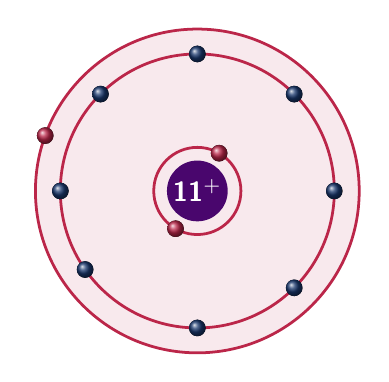
\begin{tikzpicture}[declare function ={r1=35pt;r2=110pt;r3=130pt;k=.45;}]
		\path (0:0) coordinate (O);
		\path[draw=\maunhan,fill= \maunhan!10, line width=1pt] 
		(O) circle (k*r3) 
		(O) circle (k*r2) 
		(O) circle (k*r1)
		;
		\path (O) node [shape =circle , inner sep =1pt,font=\color{white}\bfseries\sffamily,fill=\mauphu]{11$^\mathbf{+}$};
		\path (60:k*r1) node {\tikz{\fill[ball color =\maunhan] circle(3pt);}}
		(240:k*r1) node {\tikz{\fill[ball color =\maunhan] circle(3pt);}}
		(90:k*r2) node {\tikz{\fill[ball color =\maudam] circle(3pt);}}
		(-90:k*r2) node {\tikz{\fill[ball color =\maudam] circle(3pt);}}
		(0:k*r2) node {\tikz{\fill[ball color =\maudam] circle(3pt);}}
		(180:k*r2) node {\tikz{\fill[ball color =\maudam] circle(3pt);}}
		(135:k*r2) node {\tikz{\fill[ball color =\maudam] circle(3pt);}}
		(-45:k*r2) node {\tikz{\fill[ball color =\maudam] circle(3pt);}}
		(45:k*r2) node {\tikz{\fill[ball color =\maudam] circle(3pt);}}
		(215:k*r2) node {\tikz{\fill[ball color =\maudam] circle(3pt);}}
		(-200:k*r3) node {\tikz{\fill[ball color =\maunhan] circle(3pt);}}
		;
	\end{tikzpicture}
\end{document}